\documentclass{article}

\usepackage{booktabs}
\usepackage{multirow}
\usepackage{amsmath}
\usepackage{hyperref}
\usepackage{overpic}
\usepackage{amssymb}
\usepackage{graphicx}
\usepackage{tikz}
\usepackage{pgf-pie}

\usepackage[accepted]{dlai2025}

\dlaititlerunning{Audio Super-Resolution using Deep Learning - }

\begin{document}

\twocolumn[
\dlaititle{Audio Super-Resolution using Deep Learning}

\begin{center}\today\end{center}

\begin{dlaiauthorlist}
    \dlaiauthor{Kevin Cukaj}{1}
    \dlaiauthor{Cesare Corsi}{1}
\end{dlaiauthorlist}

\dlaiaffiliation{1}{University of Sapienza}

\dlaicorrespondingauthor{Kevin Cukaj}{cukaj.1942958@studenti.uniroma1.it}
\dlaicorrespondingauthor{Cesare Corsi}{corsi.2156214@studenti.uniroma1.it}


\vskip 0.3in
]

\printAffiliationsAndNotice

\begin{abstract}
This paper presents a deep learning approach for audio super-resolution.
We implement a U-Net architecture with skip connections that directly operates on raw waveforms.
Our method captures temporal and frequency characteristics of audio signals, able to reconstruct high-frequency components lost in low-resolution recordings.
Experimental results demonstrate improvements in both objective metrics and subjective quality when applied to music samples from the Free Music Archive (FMA) dataset.
\end{abstract}

% ------------------------------------------------------------------------------
\section{Introduction}

Audio super-resolution refers to the process of reconstructing high-resolution audio signals from their low-resolution counterparts. 
This task is particularly challenging because audio signals contain complex temporal and spectral features that are easily lost when downsampled to lower rates.

In this project, we address the problem of increasing the sampling rate of audio from 16 kHz to 44.1 kHz, effectively recovering the high-frequency components (above 8 kHz) that are lost in the downsampling process.
We propose a deep learning approach based on a U-Net architecture that operates directly on raw waveforms rather than time-frequency representations, allowing end-to-end training and inference without intermediate transformations.

The code for this project is available at the following GitHub repository: \url{https://github.com/KevinCukaj/deep-learning-project}.

% ------------------------------------------------------------------------------
\section{Related Work}

Multiple models such as AudioSR \cite{liu2024audiosr} (adopting a U-Net), and NU-Wave2 \cite{han2022nu} (adopting a diffusion model) were tested.
These two models were first considered as a starting point for our project.

Other possible methods for the same task include GANs and transformers.

We ultimately decided to implement our own U-Net model for direct audio super-resolution. 
Compared to transformers or diffusion models, U-Nets are easier to train, and less memory-intensive.
This also permitted more freedom in the design process.

% ------------------------------------------------------------------------------
\section{Method}

\subsection{Problem Formulation}
Let $x_{\text{LR}} \in \mathbb{R}^n$ be a low-resolution audio signal sampled at 16 kHz, and $x_{\text{HR}} \in \mathbb{R}^m$ be the corresponding high-resolution signal at 44.1 kHz, where $m > n$. Our goal is to learn a mapping function $f_\theta: \mathbb{R}^n \rightarrow \mathbb{R}^m$ such that $f_\theta(x_{\text{LR}}) \approx x_{\text{HR}}$.

\subsection{Dataset Preparation}
We create paired training examples using the Free Music Archive (FMA) dataset \cite{fma_dataset}. 
For each high-resolution audio clip $x_{\text{HR}}$, we generate its low-resolution counterpart $x_{\text{LR}}$ through the following process:
\begin{enumerate}
    \item Downsample $x_{\text{HR}}$ from 44.1 kHz to 16 kHz,
    \item Upsample back to 44.1 kHz using basic interpolation,
    \item Apply a low-pass filter with cutoff at 60\% of the Nyquist frequency (4.8 kHz). The 60\% value represents a good balance between preserving enough information for the model to learn meaningful correlations.
\end{enumerate}

This procedure simulates the bandwidth limitation of low-sampling rate audio while ensuring both signals have the same dimensions for training.

\subsection{Network Architecture}
Although U-Nets were originally designed for 2D image data, they can be adapted effectively to 1D audio waveforms by using 1D convolutional layers.

Our modified U-Net architecture consists of four encoding and decoding blocks.
The encoder path, with four convolutional layers, progressively downsamples the input while increasing feature depth (1 $\rightarrow$ 64 $\rightarrow$ 128 $\rightarrow$ 256 $\rightarrow$ 512 channels).
The decoder path uses transposed convolutions to restore the original resolution.
The architecture incorporates skip connections that concatenate corresponding encoder and decoder features, helping preserve fine-grained information that might otherwise be lost during downsampling.

Each layer uses batch normalization and appropriate activations (LeakyReLU in the encoder, ReLU in the decoder, and tanh for the output).

Simply put, the network takes as input a segment of low-resolution audio and outputs the corresponding high-resolution audio of the same length.

The model can be formalized as:
\begin{equation}
\hat{x}_{\text{HR}} = f_\theta(x_{\text{LR}})
\end{equation}

The resulting total number of parameters in the model is 5,995,457.

\subsection{Training Procedure}
As a first attempt, we used the L1-loss as our primary loss function.
Although this still produced a decent reconstruction, L1 and L2 don't reflect natural biases in human hearing since we perceive certain frequencies to be louder or quieter than others.
This is why we decided to use a perceptual loss function like STFT (Short-Time Fourier Transform) loss, which captures the frequency content of the audio signal more effectively.
The STFT loss is computed as follows:
\begin{equation}
\mathcal{L}_{\text{STFT}}(\theta) = ||\text{STFT}(f_\theta(x_{\text{LR}})) - \text{STFT}(x_{\text{HR}})||_1
\end{equation}

% ------------------------------------------------------------------------------
\section{Experimental Results}

\subsection{Implementation Details}
The model was trained on the FMA small dataset containing approximately 8,000 tracks of 30-second audio clips across various genres.
Since the computational power at our disposal was very limited, and Google Colab's free plan has its limitations, we ended up using a subset of just 2000 tracks for training.

We used an 80/10/10 split for training, validation, and testing. Training was performed on a single GPU with a batch size of 64 for 100 epochs.

The segment length (fixed-duration chunk or slice of an audio signal that is extracted and used as an input unit for a model) was set to 65536 samples (approximately 1.5 seconds at 44.1 kHz).
This was done to cope with the memory limitations of the Colab environment.

We implemented support for resuming training from previously saved checkpoints, enabling us to seamlessly continue across multiple Colab sessions and effectively bypassing session time limits.
To ensure consistency, the original dataset split used at the start of training was preserved throughout the process.

\subsection{Hyperparameter Tuning}
To find good hyperparameter values, several training runs were performed.
The final values were chosen based on the best validation loss achieved during training.  

The learning rate was initialized at 0.001, and we used the Adam optimizer with a ReduceLROnPlateau scheduler that reduces the learning rate by a factor of 0.5 when validation loss does not improve for 5 epochs.

\subsection{Evaluation Metrics}
We evaluate our model using both objective metrics and subjective evaluation:
\begin{itemize}
    \item L1 Loss: Measures the absolute difference between predicted and ground truth samples
    \item MSE Loss: Measures the squared error between predicted and ground truth samples
    \item STFT Loss: Measures the difference in frequency content between predicted and ground truth audio
    \item Qualitative assessment: human listeners evaluate the perceptual quality of the enhanced audio comparing it to the low-resolution counterpart.
\end{itemize}

\subsection{Results and Discussion}
Our model can reconstruct high-frequency components lost in low-resolution audio. 
The training process is illustrated in Figure \ref{fig:training1}, with respect to the STFT loss.

\begin{figure}[!htb]
    \centering
    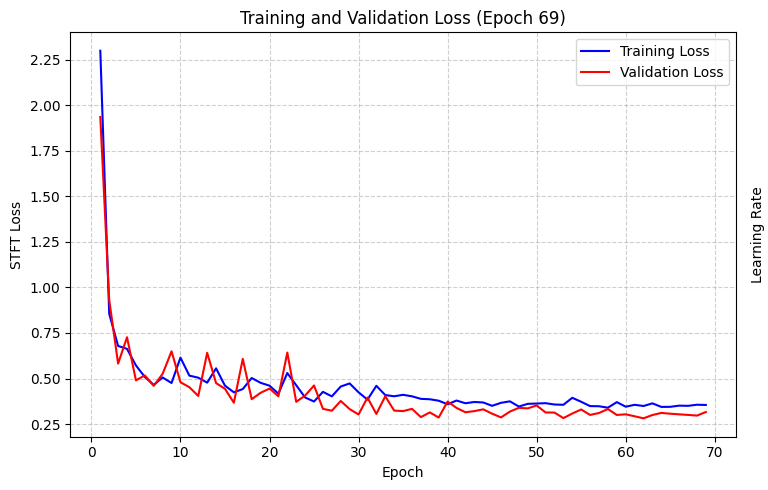
\includegraphics[width=1\linewidth]{images/training1.png}
    \vspace{-0.7cm} % Reduce space between image and caption
    \caption{Training and validation losses over epochs}
    \label{fig:training1}
\end{figure}

Although we set the training limit to 100 epochs, we decided to stop the training at epoch 69, since the validation loss plateaued, and because of diminishing returns.
Nevertheless this took around 10 hours of training across multiple sessions.

Quantitatively, we achieve the losses presented on Table \ref{tab:results1} on the test set.

\begin{table}[!htb]
    \centering
    \begin{tabular}{lc}
        \toprule
        \textbf{Metric} & \textbf{Value} \\
        \midrule
        Average L1 Loss & 0.3652 \\
        Average MSE Loss & 0.2439 \\
        Average STFT Loss & 0.3219 \\
        \bottomrule
    \end{tabular}
    \caption{Quantitative results of audio super-resolution}
    \label{tab:results1}
\end{table}

As a subjective evaluation method, MOS (Mean Opinion Score) was used, where the low resolution version and the corresponding model output of the same audio sample were given to 20 listeners.
Each had to give a score from 1 (Bad) to 5 (Excellent) based on their listening experience.
The pie chart in Figure \ref{fig:qualitative} summarizes the listeners' feedback on the restored sample.

\begin{figure}[!htb]
    \centering
    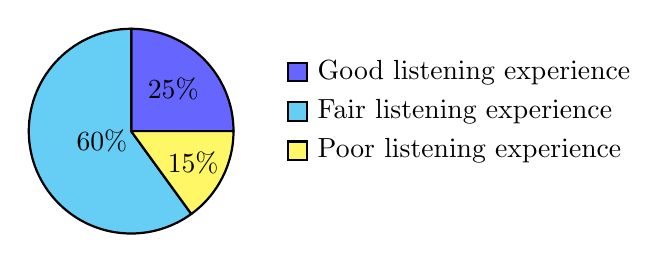
\begin{tikzpicture}
        \pie[
            radius=1.3,
            text=legend,
            after number={\%},
        ]{25/Good listening experience, 60/Fair listening experience, 15/Poor listening experience}
    \end{tikzpicture}
    \caption{Subjective evaluation of restored audio sample}
    \label{fig:qualitative}
\end{figure}

The final MOS score was
\begin{align*}
    \text{MOS} &= \frac{(5 \cdot 0) + (4 \cdot 5) + (3 \cdot 12) + (2 \cdot 3) + (1 \cdot 0)}{20} \\
    &= 3.1
\end{align*}

All of the listeners reported that the restored audio sample sounded more detailed compared to the low-resolution version.

% ------------------------------------------------------------------------------
\section{Conclusion and Future Work}

We presented a deep learning approach for audio super-resolution that is able to reconstruct high-frequency components from low-resolution audio, through a U-Net architecture that operates directly on raw waveforms.

One could possibly achieve better results by using a larger and more diverse dataset, as well as experimenting more with different combinations of hyperparameters.
Also, a longer training time could provide better results.

The primary limitation of our current approach is the segment-by-segment processing, which could introduce discontinuities at segment boundaries.
Implementing overlap-add techniques or recurrent components could address this limitation in future iterations.

% ------------------------------------------------------------------------------
\section{Appendix}

Our initial research direction focused on a multi-stage approach to audio enhancement:
\begin{enumerate}
    \item Source separation of mixed audio tracks into individual components (vocals, drums, bass, other) using the Demucs \cite{rouard2022hybrid} model.
    \item Individual enhancement of each separated track.
    \item Recombination of enhanced components into a full mix.
\end{enumerate}
We first thought that enhancing individual components separately would allow for more targeted improvements specific to each instrument type's frequency characteristics.
After a feedback from the professor's assistant, we realized that this approach might not be optimal.

We also noticed that the source separation quality was highly variable. Additionally, the processing time was significant (3-4 minutes per 3-minute track), and the phase coherence issues when recombining tracks led to noticeable artifacts.

After abandoning the source separation approach, we evaluated existing pre-trained models for direct audio enhancement:
We tested AudioSR, NU-Wave2 on our low-resolution samples.

Unfortunately, they were not suitable for our task because either the checkpoint was not available or dependencies conflicts that we could not resolve.
Also, the AudioSR model performances were not satisfactory in the Colab environment, upon which we heavily relied on for this project.
Infact, we encountered issues where we would not even get an output because of the memory limitations.

After settling with a U-Net, as a first model we trained on audio signals of 16384 samples (approximately 372 ms at 44.1 kHz), on a dataset of 1000 tracks from the FMA small dataset, on 100 total epochs.
The training took approximately 2 hours, and it is illustrated in Figure \ref{fig:training2}.
\begin{figure}[!htb]
    \centering
    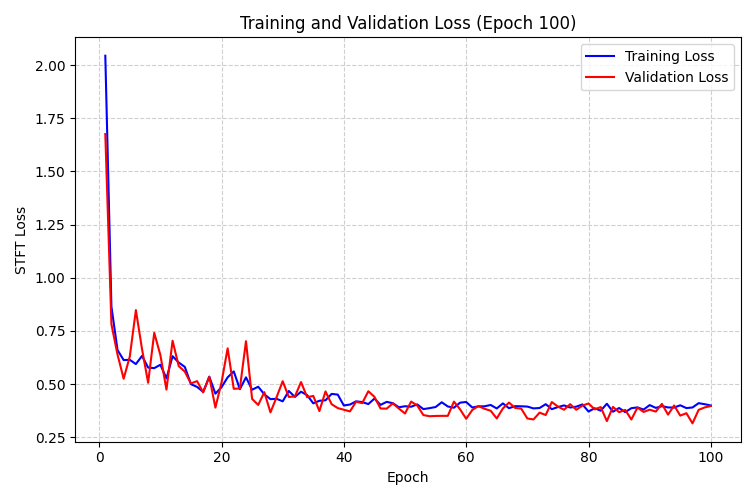
\includegraphics[width=1\linewidth]{images/training2.png}
    \vspace{-0.7cm} % Reduce space between image and caption
    \caption{Training and validation losses over epochs}
    \label{fig:training2}
\end{figure}
This resulted in the errors in Table \ref{tab:results2}.
\begin{table}[!htb]
    \centering
    \begin{tabular}{lc}
        \toprule
        \textbf{Metric} & \textbf{Value} \\
        \midrule
        Average L1 Loss & 0.4785 \\
        Average MSE Loss & 0.3805 \\
        Average STFT Loss & 0.3366 \\
        \bottomrule
    \end{tabular}
    \caption{Quantitative results of audio super-resolution}
    \label{tab:results2}
\end{table}
By analyzing the output on the inference process, we observed promising results in terms of detail preservation and artifact reduction.
Then we decided to increase the dataset size to 2000 tracks, and the audio signal segments to 65536 samples (approximately 1.5 seconds at 44.1 kHz).
This resulted in even smaller errors, which were also more significant since the dataset used was larger.
Unfortunately, we could not increase it any further since we maxed-out the VRAM on the GPU, and we had to train for several days due to Colab's session time limits, everytime resuming from a checkpoint.


\bibliography{references}
\bibliographystyle{dlai2025}

\end{document}